\subsection{Statistical Tests}

Perhaps the most important concept or theoretical underpinning of all classical statistics is the Central Limit Theorem. This theorem states that for a random sample $X_1, X_2, ..., X_n$, which is identically and independently distributed with mean $\mu$ and standard deviation $\sigma$, the sample mean is approximately distributed (converges in distribution) as such:

\begin{equation}
\bar{X} \sim N(\mu, \frac{\sigma^2}{n})
\end{equation}

\noindent where $\bar{X}$ is the sample average and as n goes to infinity.

Many of the classical significance tests are based off of this theorem. For example, say we want to understand if the true mean of a population is different than zero for some scenario. We would set up the test by first defining the null and alternative hypotheses:

\begin{equation}
\begin{split}
H_0 &: \mu = 0 \\
H_A &:  \mu \neq 0.
\end{split}
\end{equation}

\noindent Since we can't know the true population mean (we can't survey the entire population for example) we are limited to a random sample and the mean of that sample. However, we don't want to make a conclusion based solely off the sample mean alone because of the variability that is introduced by the random sample. For example, say the sample mean is 1. One conclusion (possibly false) we could make is that the population mean must be close to 1 as well and therefore we would reject the null hypothesis. It's possible however, that our sample happens to have a mean of 1 by chance whereas the population mean is really 0.

To account for this issue we use the central limit theorem to imagine a \emph{sampling distribution} where we theoretically take many, many samples of size $n$ from the original population and plot the means to form a distribution. This distribution, according to the CLT, will be distributed $N(\mu, \frac{\sigma^2}{n})$. Using our given sample or data, we temporarily make the assumption that the null hypothesis is true ($\mu=0$) and figure out how many standard deviations away our sample mean $\bar{X}$ is from $\mu=0$. This is the z-score.

Before doing this test we decide on a threshold we are comfortable with for determining if the z-score is too extreme to be due to just chance. One way to express this threshold is through critical values like 1.96 and -1.96 if doing a two-tailed test (more on those numbers in a second). If we find the z-score is greater than 1.96 or less than -1.96 in this scenario, then we can conclude that the sample mean was far enough away from 0 that it must not be due to chance alone. If we find the opposite however, then we conclude that we don't have enough evidence to reject the null hypothesis and assume our population mean is 0. 

We know that z-scores in particular are distributed normally with mean zero and variance one. Using this distribution we can calculate what is known as the p-value, or the probability we get a z-score as extreme or more extreme than the one found, assuming the null hypothesis is true. We can then compare that p-value to the probability of a z-score in general being greater than or less than our critical values, such as 1.96 and -1.96. For these values the probability is 5\% and can be written as $\alpha=0.05$, which is a common threshold chosen in academia. 

The interpretation of the p-value given above was defined in terms of the z-score, but in general it refers to the probability of getting any test statistic as extreme or more extreme than the one found, under the null hypothesis. P-values are the source of great confusion and it is important to remember the correct interpretation given above.

% TODO good to publish up to here
Table \ref{table:test_stat} below summarizes some of the basis statistical tests, followed by a more in depth discussion on each test.\newline

\begin{table}[b] \label{table:test_stat}
\begin{tabular}{|l|l|l|l|l|}
\hline
Statistical Test & When To Use & Statistic & &  \\ \hline
One sample z-test & n>30 or when we feel our sampling distribution is normal & $\frac{\bar{X} - \mu}{\frac{\sigma}{\sqrt{n}}}$  &  &  \\ \hline
One sample t-test & n<30 &  &  &  \\ \hline
Two sample z-test                      &  &  &  &  \\ \hline
Two sample t-test                      &  &  &  &  \\ \hline
Paired t-test                      &  &  &  &  \\ \hline
ANOVA                      &  &  &  &  \\ \hline
Chi-square                      &  &  &  &  \\ \hline
Kolmogorov-Smirnov                     &  &  &  &  \\ \hline
\end{tabular}
\caption{Summary of basic statistical tests}\label{table:somename}
\end{table}



\noindent \underline{\textbf{One sample z-test}}:

The equation for the one sample z-test is given by:
\begin{equation}
z = \frac{\bar{X} - \mu}{\frac{\sigma}{\sqrt{n}}}
\end{equation}

Often times $\sigma$, the population standard deviation, is not known so we instead replace it with $s$, the sample standard deviation. As a rough rule, if $n>30$, we say the sample standard deviation approximates the population standard deviation close enough and we feel more confident in treating the sampling distribution as normal. This is a rough rule so it seems when in doubt it is better to use the t-score. 

The conditions for using the z-score are therefore:
\begin{itemize}
\item Random sample
\item Independence condition (the individual observations in the sample are independent)
\item Normal condition (underlying population is normal or the sample size is large enough meaning $n>30$). If $n<30$ we need to look at the underlying data to see if the distribution is skewed or if there are outliers. If not then it may be safe to assume the sampling distribution will be normal. Note here as well that for proportions (when our original data is binary and we are doing a hypothesis test on the proportions) the test for normality is $np, n(1-p) > 10$.
\end{itemize}

\noindent \underline{\textbf{One sample t-test}}:
The equation for the one sample t-test is given by:
\begin{equation}
t= \frac{\bar{X} - \mu}{\frac{\sigma}{\sqrt{n}}}
\end{equation}

This is the same as the z-test but we use this test if we see that the population distribution is not normal and $n<30$ (as a general rule of thumb). Again if we don't know the population standard deviation we replace $\sigma$ with $s$. The other conditions (random sample and independence conditions described above) should be met as well.
\newline

\noindent \underline{\textbf{Two sample z-test}}:
Two sample tests are used to compare the means of two random and independent samples. The results are similar but instead of imagining a sampling distribution of $\bar{X}$, we instead imagine a sampling distribution of $\bar{X}_1 - \bar{X}_2$. This sampling distribution is found by first imagining the separate sampling distributions for $\bar{X}_1$ (mean $\mu_1$ and standard deviation $\frac{\sigma_1}{\sqrt{n_1}}$) and $\bar{X}_2$ (mean $\mu_2$ and standard deviation $\frac{\sigma_2}{\sqrt{n_2}}$). The mean therefore of $\bar{X}_1 - \bar{X}_2$ will be $\mu_1 - \mu_2$ and the standard deviation will be

\begin{equation}
\begin{split}
\sqrt{\text{Var}(\bar{X}_1 - \bar{X}_2)} & = \sqrt{\text{Var}(\bar{X}_1 + (- \bar{X}_2))} \\
&=\sqrt{\text{Var}(\bar{X}_1) + (-1)^2 \text{Var}(\bar{X}_2) + (-1)*2\text{Cov}(\bar{X}_1, \bar{X}_2)} \\
&=\sqrt{\text{Var}(\bar{X}_1) + \text{Var}(\bar{X}_2)}  \hspace{1em}   \text{(since $\bar{X}_1$ and $\bar{X}_2$ are independent)}\\
&=\sqrt{ \frac{\sigma_1^2}{n_1} + \frac{\sigma_2^2}{n_2}}
\end{split}
\end{equation}

Our null hypothesis will then typically be:

\begin{equation}
\begin{split}
H_0 &: \mu_1 - \mu_2 = 0 \\
H_A &:   \mu_1 - \mu_2 \neq 0
\end{split}
\end{equation}

\noindent If both samples are large enough ($n_1, n_2 > 30$) then we assume that the sampling distribution of $\bar{X}_1$ - $\bar{X}_2$ is normal and we can use the z-score:

\begin{equation}
z = \frac{(\bar{X}_1 -   \bar{X}_2) - (\mu_1 - \mu_2)}{\sqrt{\frac{s_1^2}{n_1} + \frac{s_2^2}{n_2}}}.
\end{equation}

\noindent \underline{\textbf{Two sample t-test (variances are different)}}:

If the one of the sample sizes is below 30 then it is best to use the t-test. The score below is used when the variances are different. This is known as Welch's t-test:

\begin{equation}
t = \frac{(\bar{X}_1 -   \bar{X}_2) - (\mu_1 - \mu_2)}{\sqrt{\frac{s_1^2}{n_1} + \frac{s_2^2}{n_2}}}.
\end{equation}

\noindent \underline{\textbf{Two sample t-test (variances are same)}}:

\begin{equation}
t = \frac{(\bar{X}_1 -   \bar{X}_2) - (\mu_1 - \mu_2)}{s_p\sqrt{\frac{1}{n_1} + \frac{1}{n_2}}}.
\end{equation}

This image \ref{fig:stats_tests_diagram} is gold when trying to determine which test to use (taken from \href{https://bloomingtontutors.com/blog/when-to-use-the-z-test-versus-t-test}{here}).


 \begin{figure} \label{fig:stats_tests_diagram}
\caption{Stats test diagram}
\centering
 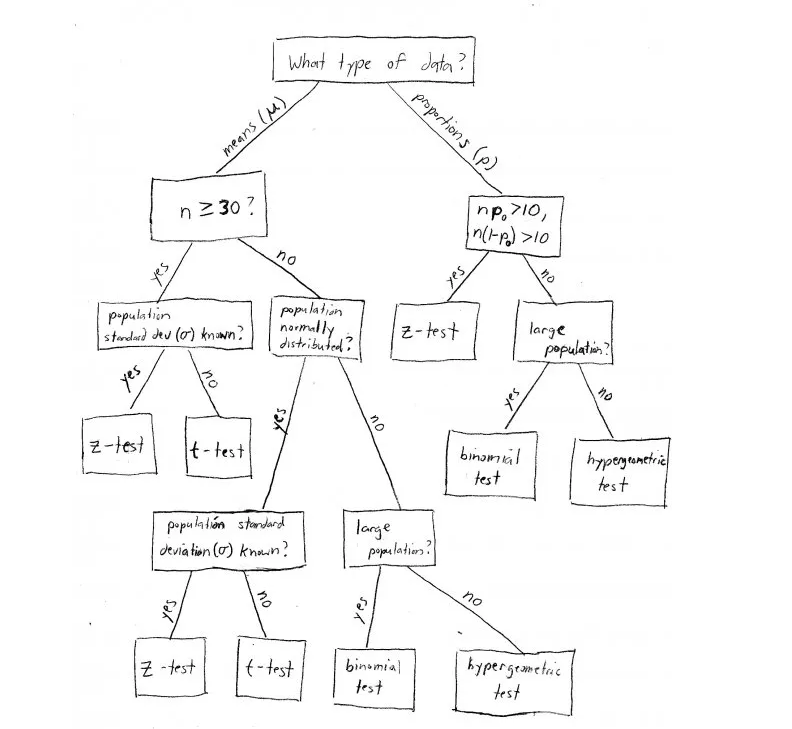
\includegraphics[scale=.3]{stats_tests.png}
 \end{figure}


\subsection{Analysis of Variance (ANOVA)}

The previous test statistics are for when we want to compare a sample mean with some value or when we want to compare two sample means with each other. Analysis of Variance comes into play when we want to compare multiple samples (3 or more). 




\subsection{Power Analysis}

Power is simply the probability that we get a test statistic more extreme than our critical value, assuming our alternative hypothesis is true - or maybe better said the probability we reject the null hypothesis given our alternative is true. 

To better see what this looks like consider a simple one-sample t-test where our null hypothesis and alternative hypothesis are defined by:

\begin{equation}
\begin{split}
H_0 &: \mu = 0 \\
H_A &:  \mu > 0.
\end{split}
\end{equation}

\noindent Power is then defined as:

\begin{equation}
P(t > c | \mu = \theta) = \text{power}.
\end{equation}

Involved in this equation are four parameters we are concerned with, namely the power, the effect size (represented as $\theta$ in this case since our null hypothesis is that $\mu=0$), the critical value $c$ (determined by our selection of $\alpha$ in our test), and the sample size (part of the test statistic $t$). 

So for example, say we get a sample mean of $\bar{X}$ with a standard deviation $s$ and sample size 10. Our t-statistic will be:

\begin{equation}
t = \frac{\bar{X} - 0}{\frac{s}{\sqrt{10}}}
\end{equation}
\noindent Since we don't know the true standard deviation, and because our sample size is low, then we know this follows a t distribution with degrees of freedom 9. Therefore, if we choose $\alpha=0.05$, the critical value will be around 1.833 from a standard t-table. The probability 

\begin{equation}
P \left( \frac{\bar{X} - 0}{\frac{s}{\sqrt{10}}}> 1.833 \right) 
\end{equation}
\noindent would give us our p-value, since this is assuming our null is true ($\mu=0$). However, for power we assume that the alternative is true for some effect size. For example if 1 is the effect size then we have:

\begin{equation}
\begin{split}
P \left( \frac{\bar{X} - 0}{\frac{s}{\sqrt{10}}} > 1.833 | \mu = 1 \right)  & = P \left(\frac{\bar{X} - 1+1}{\frac{s}{\sqrt{10}}} > 1.833 | \mu = 1 \right) \\
&= P \left( \frac{\bar{X} - 1}{\frac{s}{\sqrt{10}}} > 1.833 - \frac{1}{\frac{s}{\sqrt{10}}}  | \mu = 1 \right) \\
&= 1 - P \left( \frac{\bar{X} - 1}{\frac{s}{\sqrt{10}}}< 1.833 - \frac{1}{\frac{s}{\sqrt{10}}}  | \mu = 1 \right) \\
\end{split}
\end{equation}
\noindent which is 1 minus the cdf of the standard t-distribution. What happened here is that as soon as we assumed the alternative was true ($\mu=1$) then we needed to re-standardize the t-statistic to get back at the standard t-distribution.

This final line shows us the relationship between power, sample size, effect size, and the critical value. For example, if our effect size (1 in this case) were to be larger, then 1 minus the cdf would be larger and therefore the power would be larger indicating the fact that with a larger true effect size we are more confident in correctly rejecting the null. Another example would be if we increase the sample size (10 in this case) to a larger number. As this number increases, the same result occurs, and we are more confident in correctly rejecting the null. 

This is an important issue to consider in the realm of big data because with lots of data we will almost surely reject the null because our power is so high, even though the effect size might be fairly miniscule. It's almost as if the sheer amount of data overwhelms the effect size in the formula. For example, imagine we take a small sample of 20 people and find that those who take some treatment have an extremely small positive improvement, but our statistical test comes back without enough evidence to reject the null. If we keep all else the same and only increase sample size and find the same effect size, we most likely will reject the null just because of the fact we have more samples which increases our power. The thing to keep in mind however, is that the effect size is the same in both cases and may not be meaningful. 







